\section{How it Works}

	\subsection{Grayscale Square Images}

		We will first try our hands upon a grayscale images. Grayscale images are images in which every pixel has a single brightness value. So it is easier to work with.
		
		After Importing all the classes and functions\footnote{All the relevant functions and classes have been kept in: \href{https://github.com/PeithonKing/comp_phys_P346/blob/main/library/DIY.py}{\textbf{the Library File}}} from the library file, we can make an instance of the \href{https://github.com/PeithonKing/comp_phys_P346/blob/main/library/DIY.py#L62-L84}{\texttt{GrayscaleImageSVD()}} class. This class takes the location of the image as an input. When the instance is constructed, it loads the image to it's memory as a numpy array. Then it callculates the U, S and V matrices using the \href{https://numpy.org/doc/stable/reference/generated/numpy.linalg.svd.html}{\texttt{numpy.linalg.svd()}} function from the \href{https://numpy.org/}{\textbf{NumPy}} library.
		\vspace{-2mm}

		\begin{center}
			\noindent\fbox{
				\parbox{0.95\columnwidth}{
				\textbf{Using \href{https://numpy.org/doc/stable/reference/generated/numpy.linalg.svd.html}{\texttt{numpy.linalg.svd()}} function:} We can use the \href{https://numpy.org/doc/stable/reference/generated/numpy.linalg.svd.html}{\texttt{numpy.linalg.svd()}} function to compute the SVD of a matrix. The function returns the $3$ matrices: $U$, $S$ and $V$. In the $S$ matrix, we get the singular values in descending order. The function returns the matrix $S$ not in the form of a diagonal matrix but as a vector of singular values. So, we will have to convert it into a diagonal matrix (by \href{https://numpy.org/doc/stable/reference/generated/numpy.diag.html}{\texttt{numpy.diag()}} function) before we can use it to reconstruct the matrix $A$.
				}
			}
		\end{center}

		\begin{lstlisting}[language=Python, caption={Creating GrayscaleImageSVD class}]
	from library.DIY import GrayscaleImageSVD, show_image
	pic = "monkey"
	img = GrayscaleImageSVD(f"static/{pic}.jpg")
	img.display("Original Square Grayscale Image")\end{lstlisting}
		
		\begin{figure}[H]
			\centering
			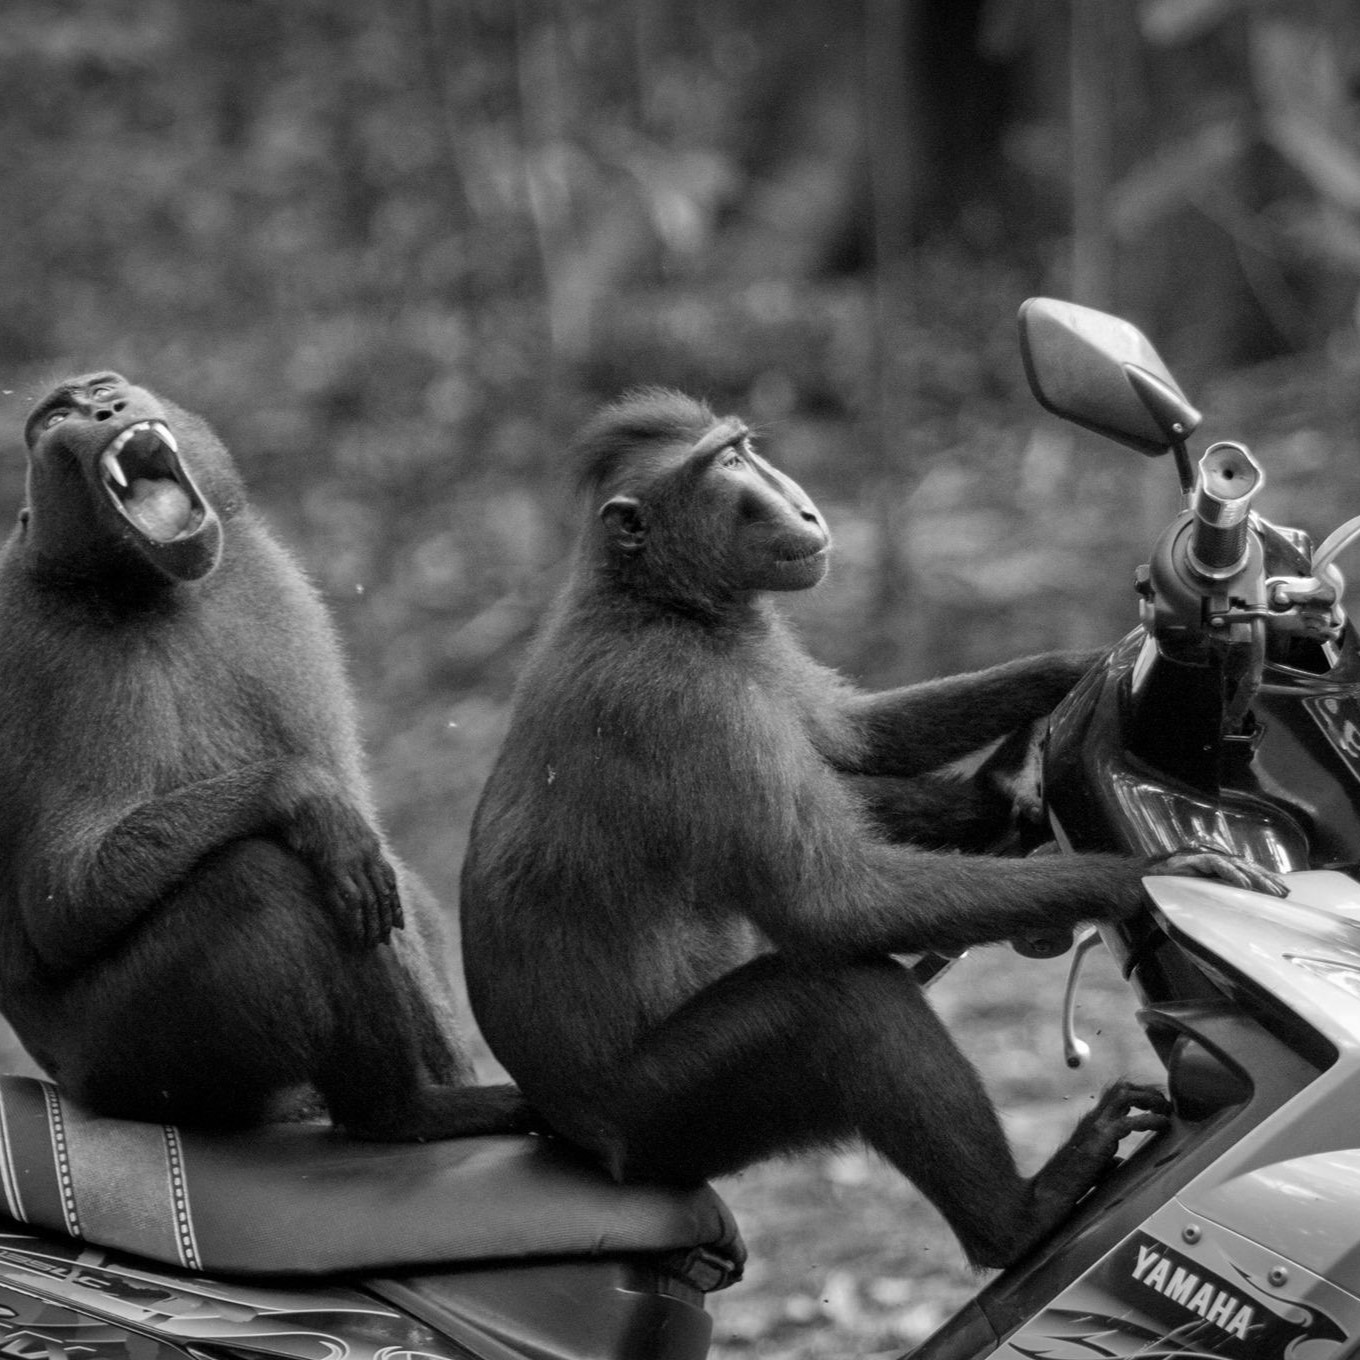
\includegraphics[width=0.35\textwidth]{../static/monkey.jpg}
			\caption{Original Square Grayscale Image}
			\label{fig:g_monkey_orig}
		\end{figure}

		Next, we can call the \href{https://github.com/PeithonKing/comp_phys_P346/blob/main/library/DIY.py#L70-L75}{\texttt{GrayscaleImageSVD.reduce()}} method to get the reduced image. This function takes the number of singular values to be used as an input. It then uses the first $n$ singular values to reconstruct the image. The function returns the reconstructed image as a numpy array. We can then use the \href{https://github.com/PeithonKing/comp_phys_P346/blob/main/library/DIY.py#L19-L31}{\texttt{show\_image()}} function to display the image. Note that, the returned array is not smaller in size than the original image; it is a full sized image. But this array can be constructed using arrays of much smaller sizes.

		Although we have writen our own \texttt{SVD()} function \href{https://github.com/PeithonKing/comp_phys_P346/blob/main/DIY%20Project/trying_SVD.ipynb}{(demonstration \textbf{here})}, we won't be actually using that for this project.

		\begin{center}
			\noindent\fbox{
				\parbox{0.95\columnwidth}{
					\textbf{Why are we using the SVD function from numpy and not using the \texttt{SVD()} function which is our own?}
					This is because the \texttt{SVD()} function from numpy takes it back to C for doing the calculations and is highly optimized. So, it is much faster than our own implementation (our function is almost 2x slower than the numpy implementation). Moreover finding SVD of a matrix involves finding eigenvalues and eigenvectors of the matrix. We know that the algorithms studied in this class become inefficient if we are working with a large matrix. The later values have a lot of error in them. So, writing the \texttt{SVD()} function is itself a huge problem to be solved. On the other hand, \textbf{finding SVD of a matrix is a very well studied problem in literature} and there are many efficient algorithms to find it. So, we can use the \texttt{numpy.linalg.svd()} function from numpy without reinventing the wheel.
				}
			}
		\end{center}

		\begin{lstlisting}[language=Python, caption={Reducing the image}, label={lst:g_monkey_10}]
	n_terms = 10  # taking upto 10 terms
	A2, ratio, error = img.reduce(terms = n_terms)
	print(f"size = {ratio}% of original image")
	print(f"RMS deviation in pixel values from the original is: {error}")
	show_image(A2)\end{lstlisting}

		\begin{figure}[H]
			\centering
			\fbox{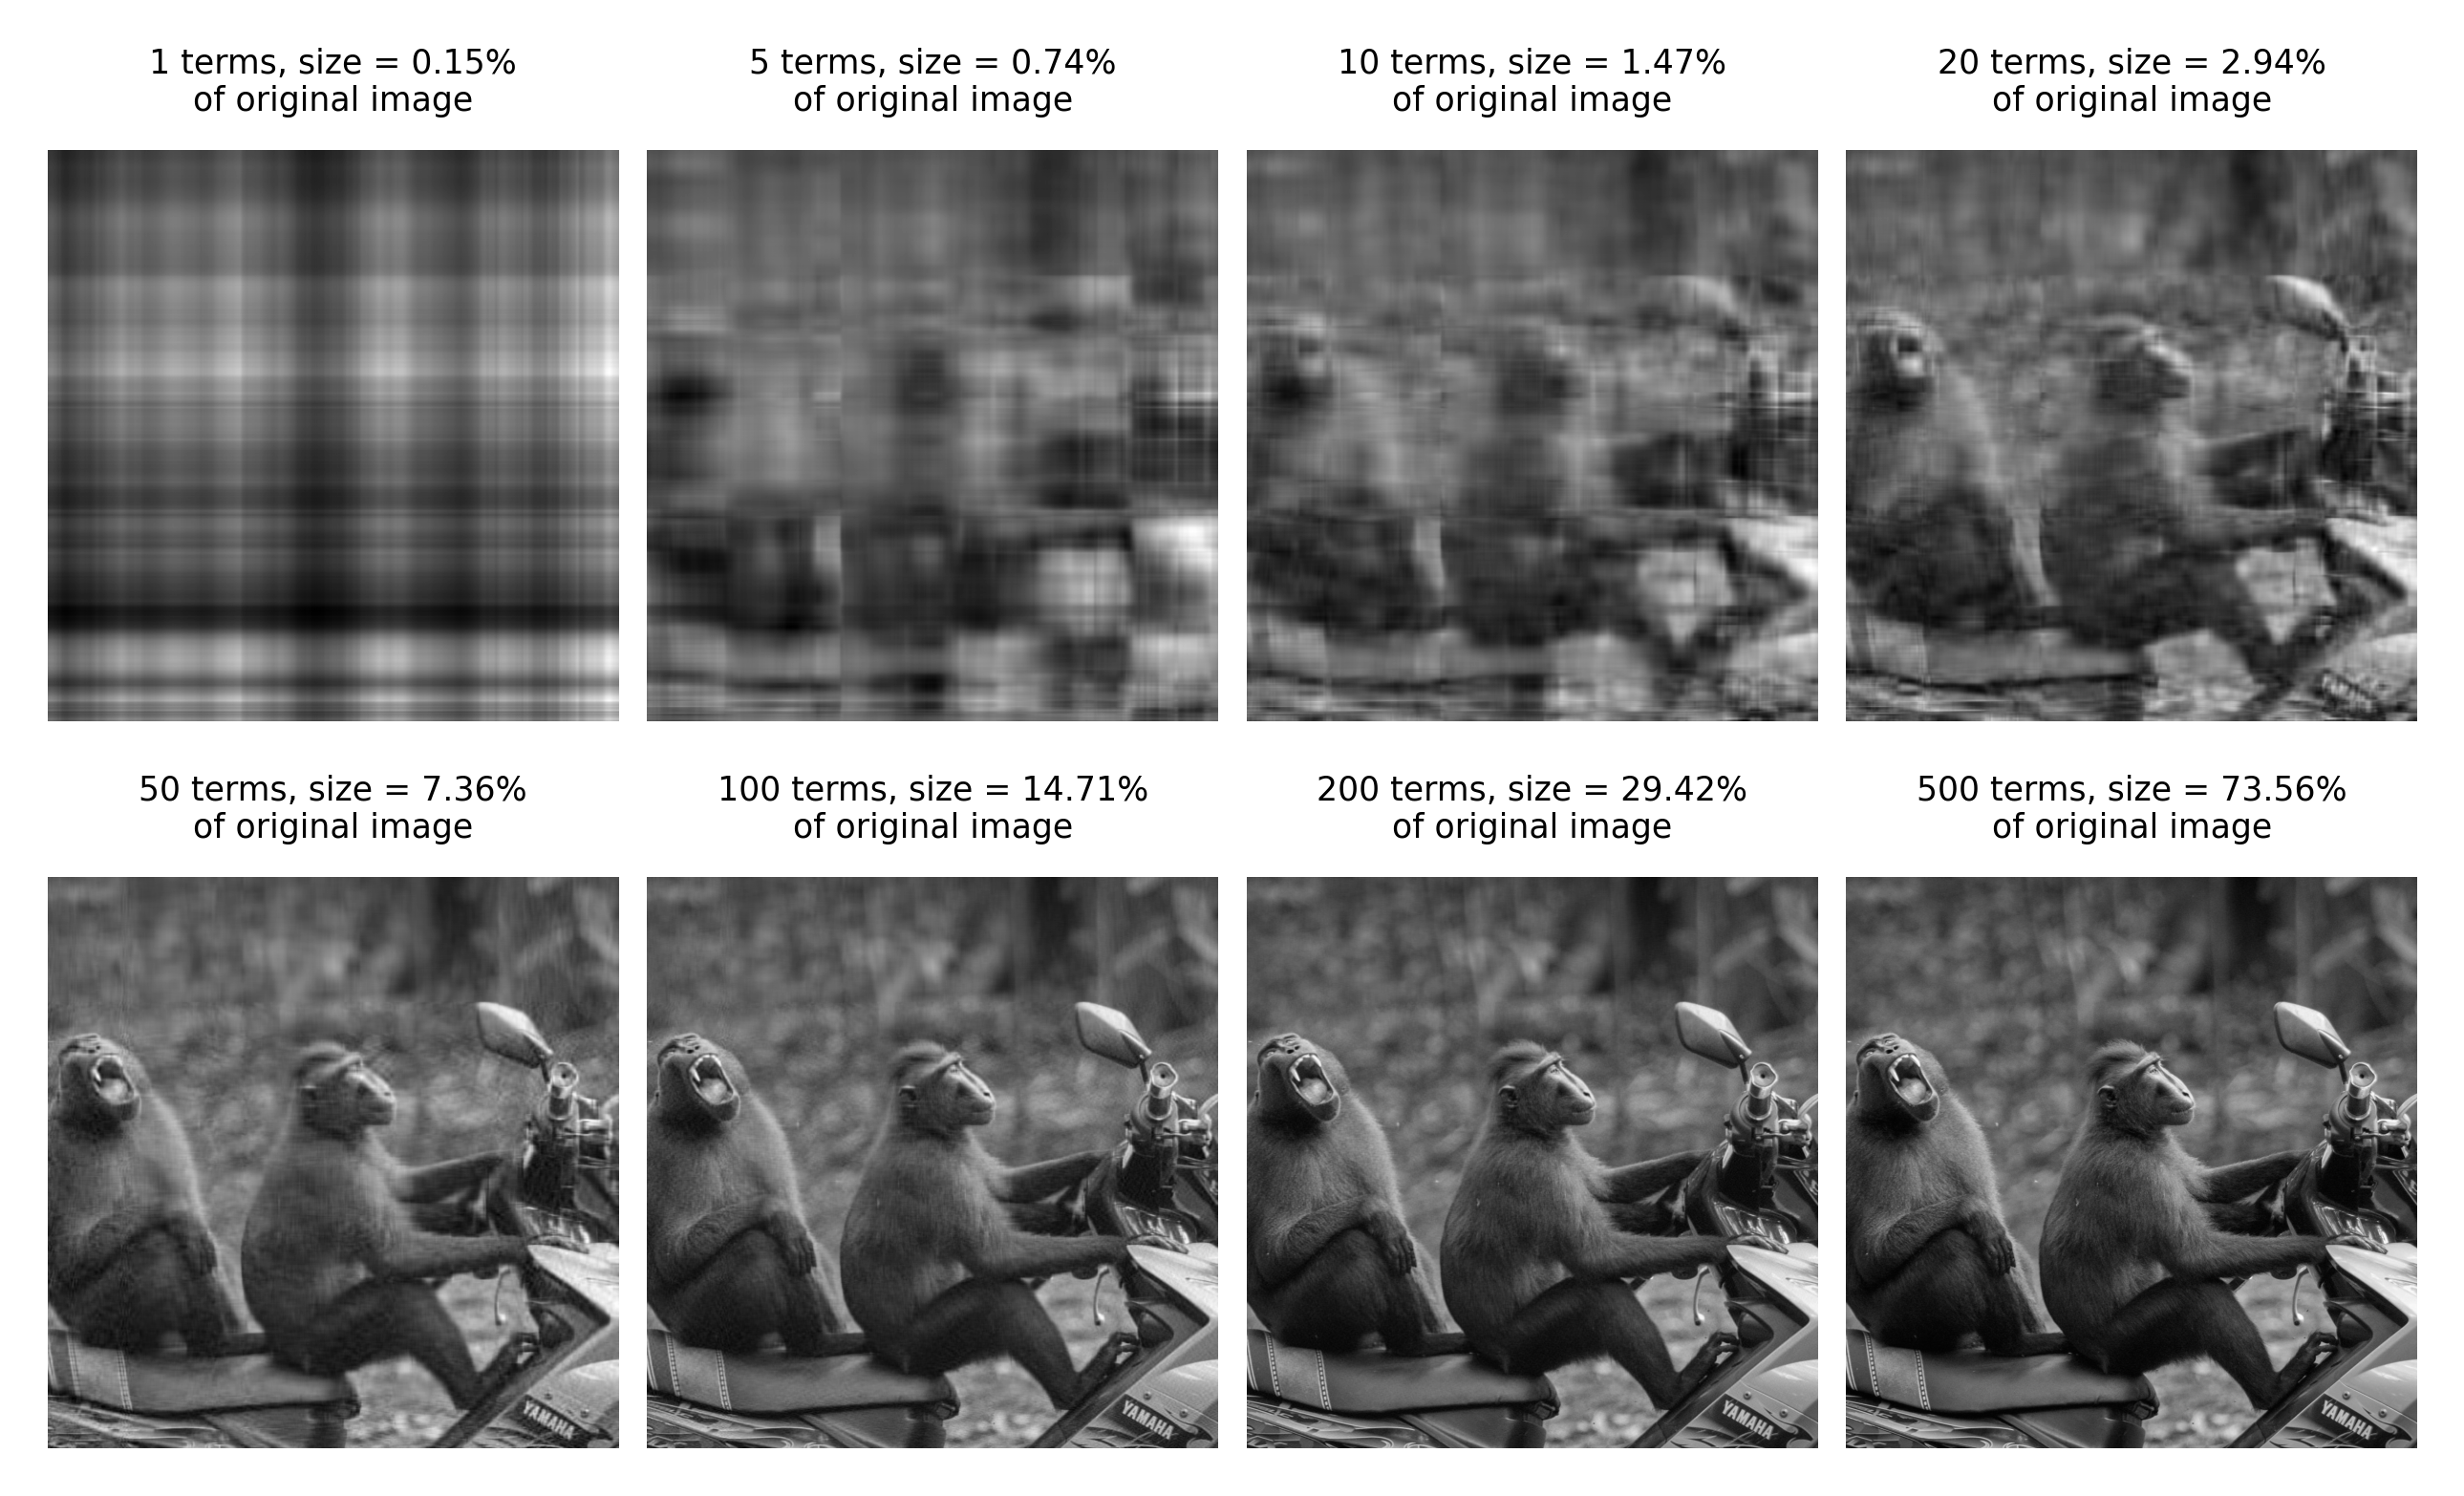
\includegraphics[width=0.45\textwidth]{../static/monkey_evolution.png}}
			\caption{\href{https://github.com/PeithonKing/comp_phys_P346/blob/main/static/monkey_evolution.png}{\textbf{Reduced image comparison with different number of terms and sizes}}.}
			\label{fig:g_monkey_evol}
		\end{figure}

		(Above comparison image might be of low quality. Find HD version \href{https://github.com/PeithonKing/comp_phys_P346/blob/main/static/monkey_evolution.png}{\textbf{here}}.)

		\subsubsection{Discussion}

			As we can clearly see from the images above, our image compression is a tradeoff with quality of the image. So, how many terms should we take? The answer to this question solely depends upon the application.

			\begin{itemize}
				\item \textbf{1 term:} We can only see some illuminated lines in the image.
				\item \textbf{5 terms:} Now, the image definitely contains more information, but no clear structure can be seen.
				\item \textbf{10 terms:} Now, we can see some structure in the image. But the image is still very noisy.
				\item \textbf{20 terms:} Now, the structures in the image are more clear. One can tell that it is a monkey riding a scooty.
				\item \textbf{50 terms:} At this point, the image is pretty clear. The name on the scooty is also readable, but the image lacs details.
				\item \textbf{100 and 200 terms:} The background becomes less noisy. Details like individual strands of hair become clearer.
				\item \textbf{500 terms:} This image is almost as good as the original image. No difference can be seen on the picture alone. If one compares it side by side with the original image, they can easily spot a difference in the contrast of the two images.
			\end{itemize}

	\subsection{Grayscale Rectangular Images}
		The \href{https://github.com/PeithonKing/comp_phys_P346/blob/main/library/DIY.py#L62-L84}{\texttt{GrayscaleImageSVD()}}  function is a generalised one. It works on both square and rectangular grayscale images. Let's see how it looks on a rectangular image.

		The original lion image can be found \href{https://github.com/PeithonKing/comp_phys_P346/blob/main/static/lion.jpg}{\textbf{here}}.

		\begin{figure}[H]
			\centering
			\fbox{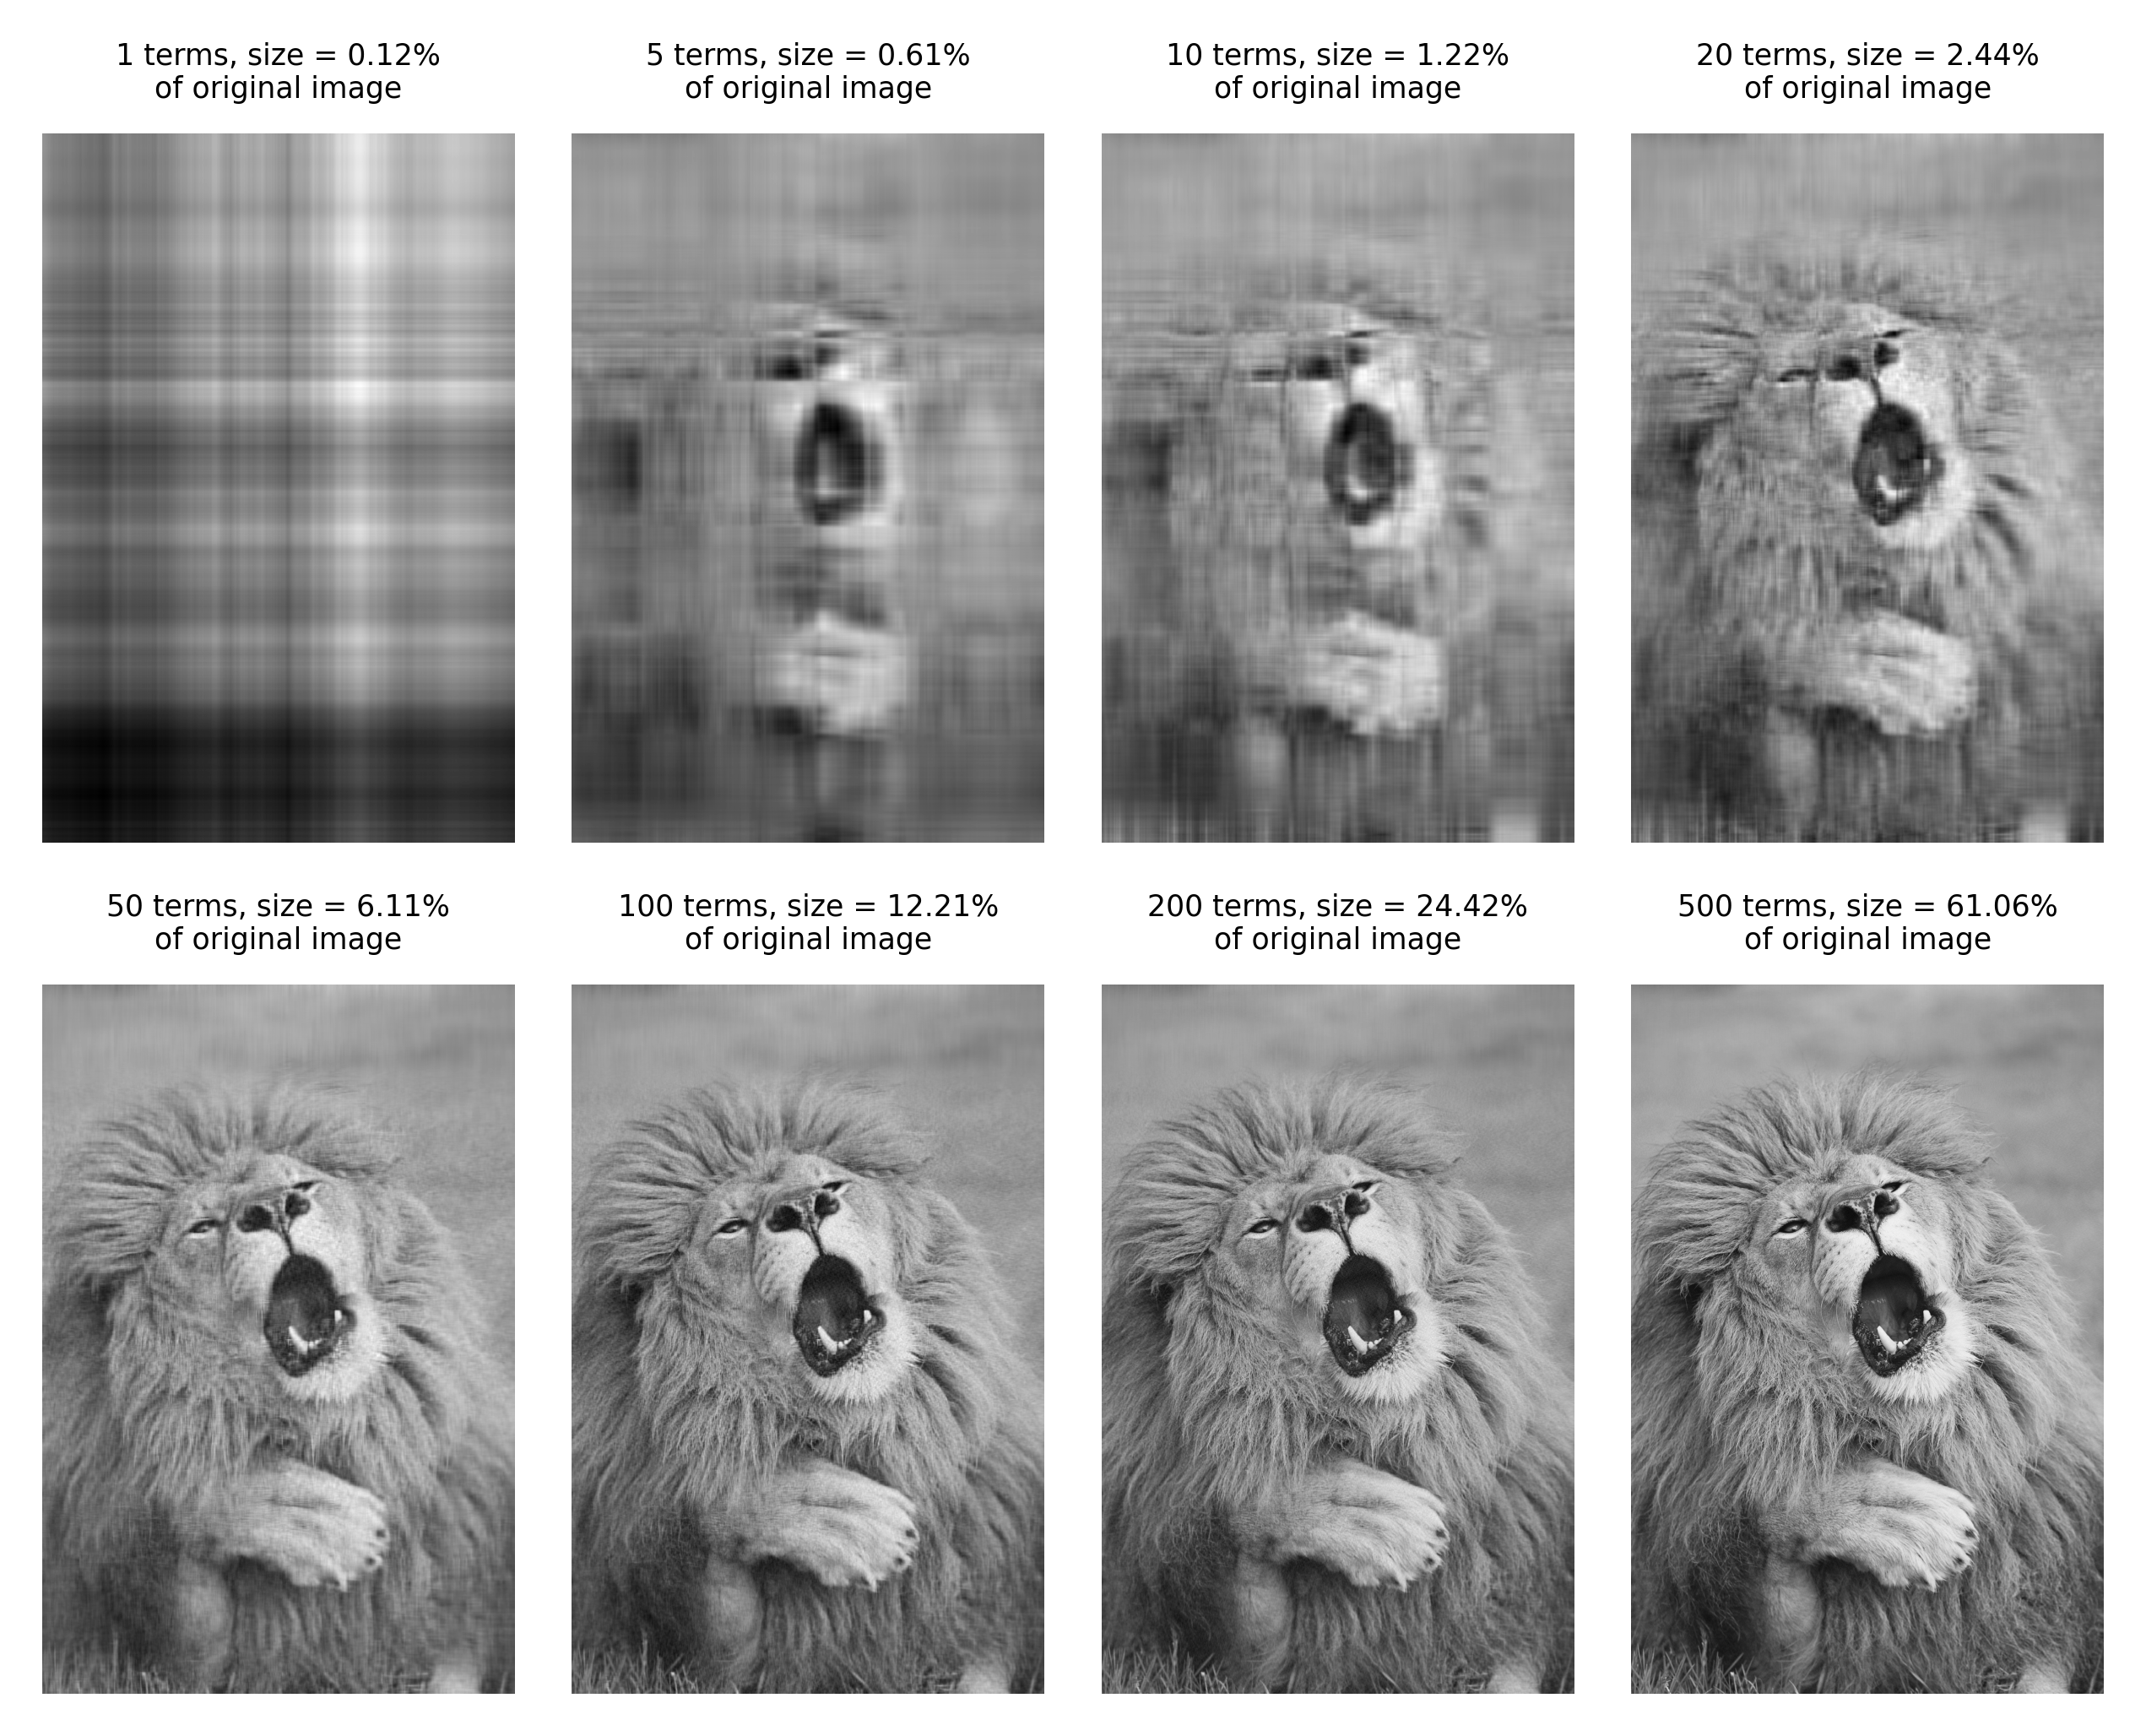
\includegraphics[width=0.4\textwidth]{../static/lion_evolution.png}}
			\caption{\href{https://github.com/PeithonKing/comp_phys_P346/blob/main/static/lion_evolution.png}{\textbf{Reduced rectangular image comparison with different number of terms and sizes}}.}
			\label{fig:g_lion_evol}
		\end{figure}

		(Above comparison image might be of low quality. Find HD version \href{https://github.com/PeithonKing/comp_phys_P346/blob/main/static/lion_evolution.png}{\textbf{here}}.)

	\subsection{Color Images}

		Colour images consist of 3 channels of data: Red, Green and Blue. So, for colour images we need to perform SVD on each channel separately. The \href{https://github.com/PeithonKing/comp_phys_P346/blob/main/library/DIY.py#L86-L133}{\texttt{ColourImageSVD()}} class does exactly that. Let's see how it looks on a color image.

		\begin{lstlisting}[language=Python, caption={Working with colour images}, label={lst:c_crab_10}]
		import library.DIY as DIY
		img = DIY.ColourImageSVD(f"static/crab.jpg")
		img.display("Original Square Grayscale Image")
		A2, ratio, error = img.reduce(terms = 10)
		DIY.show_image(A2)\end{lstlisting}

		\begin{figure}[H]
			\centering
			\fbox{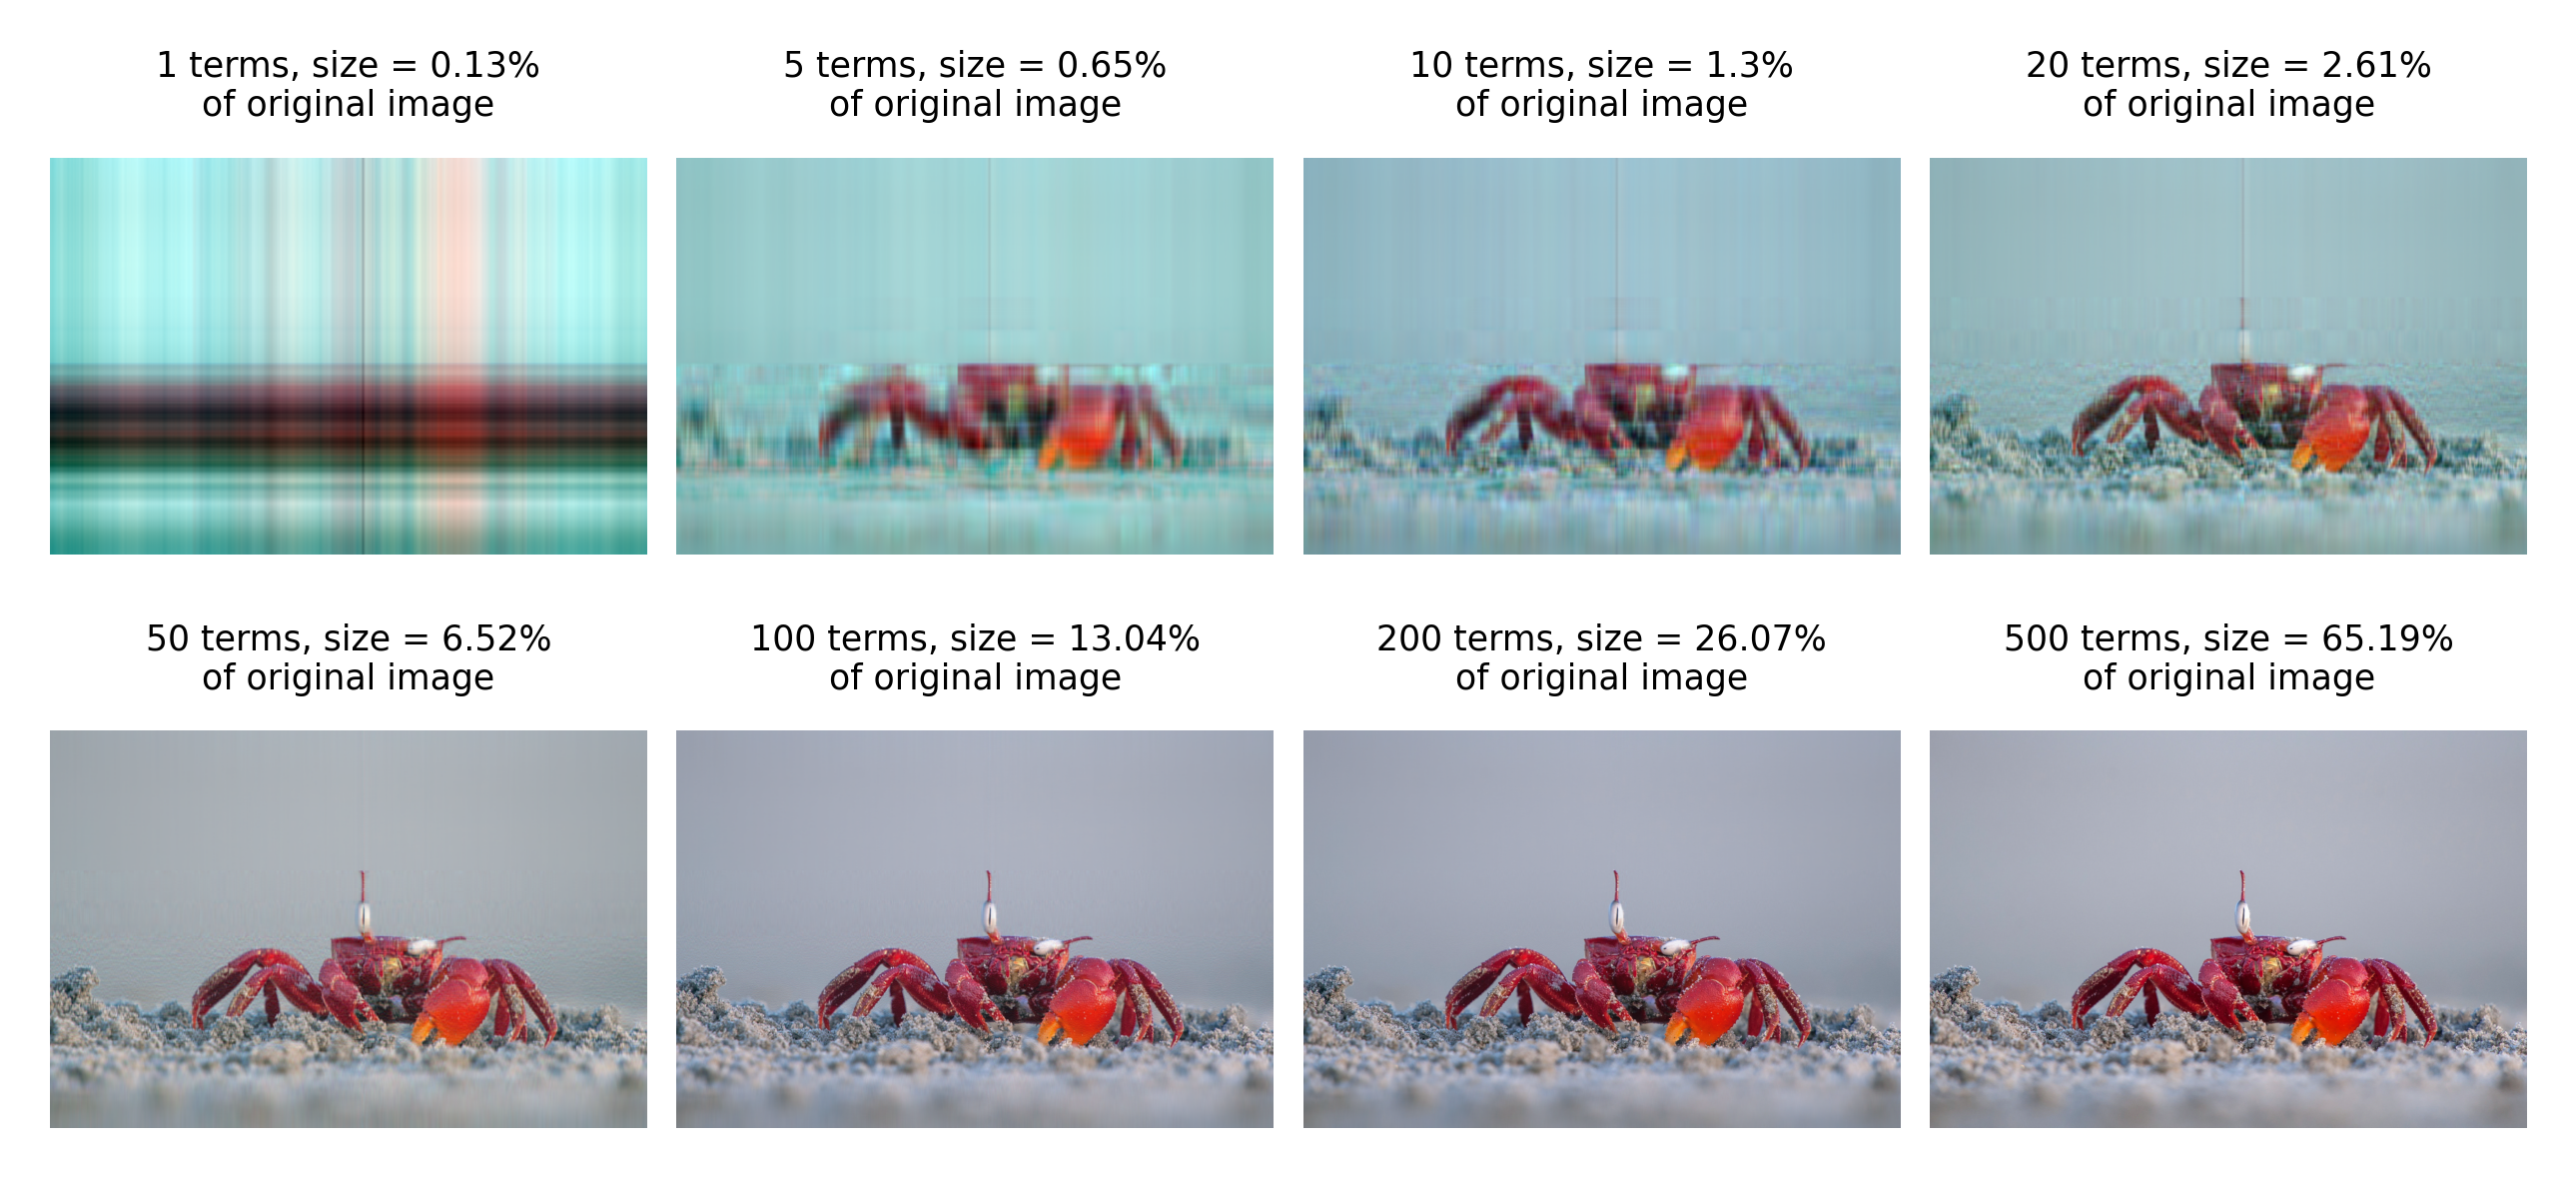
\includegraphics[width=0.45\textwidth]{../static/crab_evolution.png}}
			\caption{\href{https://github.com/PeithonKing/comp_phys_P346/blob/main/static/crab_evolution.png}{\textbf{Reduced colour image comparison with different number of terms and sizes}}.}
			\label{fig:c_crab_evol}
		\end{figure}

		(Above image might be of low quality. Original image can be found \href{https://github.com/PeithonKing/comp_phys_P346/blob/main/static/crab_evolution.png}{\textbf{here}}.)
